\subsubsection{Candidate Assertions} \label{Sec:candidateAssertions}
\IncMargin{0em}
\begin{algorithm}[t]
{\scriptsize
\SetKwInOut{Input}{input}\SetKwInOut{Output}{output}
\Input{Test suite $T$; The set of test cases $tc_i \in T$}
\Output{The ordered set of oracles $oracles$}
\BlankLine

\Begin {
\nl \For{$tc_i \in T$}{
\nl  $trace \leftarrow textsc{Exec}(tc_i)$\\
\nl  $domAccss \leftarrow \textsc{GetDOMAcc}(trace)$\\   	
\nl  $freqAccdDOM\leftarrow \emptyset$\\
\nl  \For{$dom \in domAccss $}{
\nl   \If{$\textsc{DOMUsgFreq}(dom) \geq \frac{1}{NoOfDOMElems} $}{
\nl    $freqAccdDOM \leftarrow dom \cup freqAccdDOM$\\       
      }
     }
\nl  \For{$asstn \in assertions_{tc_i}$}{
\nl   $asserDOMAcc \leftarrow \textsc{GetDOMAcc}(asstn)$\\
\nl   $asserDOMMuts \leftarrow \textsc{GetDOMMuts}(asserDOMAcc)$\\
\nl   \For{$domMut \in asserDOMMuts$}{
\nl    $bwSts \leftarrow \textsc{GetBWSlice}(domMut, trace)$\\
\nl    $asstnRel \leftarrow \textsc{GetWrVars}(bwSts)$\\
\nl    $potAsstnRel \leftarrow \textsc{GetFWSlice}(asstnRel, trace)$\\
      }
     }
\nl  $nonAsserDOMMuts \leftarrow \textsc{GetDOMMuts}(freqAccdDOM)$\\
\nl  \For{$domMut \in nonAsserDOMMuts$}{
\nl   $bwSts \leftarrow \textsc{GetBWSlice}(domMut, trace)$\\
\nl   $nonAsstnRel \leftarrow \textsc{GetWrVars}(bwSts)$\\
     }
\nl  $asstnRelOrcls[func]_{f=1}^{n} \leftarrow \textsc{GetValue}(\textsc{Accessibles}([func]_{f=1}^{n}, asstnRel))$\\
\nl  $candidOrcls[func]_{f=1}^{n} \leftarrow \textsc{Accessibles}([func]_{f=1}^{n}, [potAsstnRel \cup nonAsstnRel])$\\
\nl  $oracles[func]_{f=1}^{n}.\textsc{Add}(asstnRelOrcls \cup candidOrcls)$\\
   }
\nl $\textsc{Rank}(oracles[func]_{f=1}^{n})$\\
\nl return $(oracles[func]_{f=1}^{n})$
}
\caption{Oracle Generation} 
\label{Alg:algorithm}
}
\end{algorithm}
%\DecMargin{lem}
\begin{figure}[!t]
  \centering
  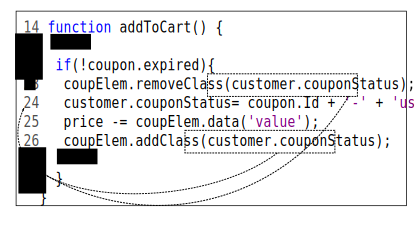
\includegraphics[width=.9\hsize]{fig/candidateDOMToCode}
  \mycaption{Relating candidate DOM element to \javascript code.}
  \vspace{-0.1in} 
  \label{Fig:candidateDOMToCode}
  \vspace{-0.1in} 
\end{figure}
In addition to explicit and implicit assertions, we also verify the correctness of code-level entities pertaining to DOM updates, which are essentially important but not checked in the existing DOM-based test cases. We derive such unit-level assertions, namely candidate assertions, from the candidate DOM element properties previously obtained from the test case execution (box 3 in \figref{approachDiagram}). As the test case runs, we monitor DOM's evolution and match the list of mutated DOM elements and their properties with property updates of the candidate DOM elements. Once a match is found, we infer backwards slice statements pertaining to the mutation of DOM element's property (\textsc{GetBWSlice} in line 18 of the algorithm). Therefore, in this case the slicing criteria which is given as input to the backwards slicing module is an update to the property of the candidate DOM element.
After gathering the related \javascript statements within the application, we extract accessible entities of these statements (\textsc{Accessibles} in line 22) which form our candidate assertions. $candidateAsstn$ in line 22 contains our candidate assertions. 

Recall from the example (\figref{example}), one such potential DOM property which we record as part of \secref{extractDomRelatedInfo}, is \code{class} attribute associated with DOM element with ID \code{couponButt}. Monitoring DOM changes reveal that line 26, where the \code{class} attribute of the element is set, is the initial point of contact between DOM mutation and the \javascript code. Given line 26 as the slicing criteria, \code{customer.couponStatus} (line 24) is marked as the candidate assertion.